% Options for packages loaded elsewhere
\PassOptionsToPackage{unicode}{hyperref}
\PassOptionsToPackage{hyphens}{url}
%
\documentclass[
  doc,floatsintext]{apa6}
\usepackage{amsmath,amssymb}
\usepackage{iftex}
\ifPDFTeX
  \usepackage[T1]{fontenc}
  \usepackage[utf8]{inputenc}
  \usepackage{textcomp} % provide euro and other symbols
\else % if luatex or xetex
  \usepackage{unicode-math} % this also loads fontspec
  \defaultfontfeatures{Scale=MatchLowercase}
  \defaultfontfeatures[\rmfamily]{Ligatures=TeX,Scale=1}
\fi
\usepackage{lmodern}
\ifPDFTeX\else
  % xetex/luatex font selection
\fi
% Use upquote if available, for straight quotes in verbatim environments
\IfFileExists{upquote.sty}{\usepackage{upquote}}{}
\IfFileExists{microtype.sty}{% use microtype if available
  \usepackage[]{microtype}
  \UseMicrotypeSet[protrusion]{basicmath} % disable protrusion for tt fonts
}{}
\makeatletter
\@ifundefined{KOMAClassName}{% if non-KOMA class
  \IfFileExists{parskip.sty}{%
    \usepackage{parskip}
  }{% else
    \setlength{\parindent}{0pt}
    \setlength{\parskip}{6pt plus 2pt minus 1pt}}
}{% if KOMA class
  \KOMAoptions{parskip=half}}
\makeatother
\usepackage{xcolor}
\usepackage{color}
\usepackage{fancyvrb}
\newcommand{\VerbBar}{|}
\newcommand{\VERB}{\Verb[commandchars=\\\{\}]}
\DefineVerbatimEnvironment{Highlighting}{Verbatim}{commandchars=\\\{\}}
% Add ',fontsize=\small' for more characters per line
\usepackage{framed}
\definecolor{shadecolor}{RGB}{248,248,248}
\newenvironment{Shaded}{\begin{snugshade}}{\end{snugshade}}
\newcommand{\AlertTok}[1]{\textcolor[rgb]{0.94,0.16,0.16}{#1}}
\newcommand{\AnnotationTok}[1]{\textcolor[rgb]{0.56,0.35,0.01}{\textbf{\textit{#1}}}}
\newcommand{\AttributeTok}[1]{\textcolor[rgb]{0.13,0.29,0.53}{#1}}
\newcommand{\BaseNTok}[1]{\textcolor[rgb]{0.00,0.00,0.81}{#1}}
\newcommand{\BuiltInTok}[1]{#1}
\newcommand{\CharTok}[1]{\textcolor[rgb]{0.31,0.60,0.02}{#1}}
\newcommand{\CommentTok}[1]{\textcolor[rgb]{0.56,0.35,0.01}{\textit{#1}}}
\newcommand{\CommentVarTok}[1]{\textcolor[rgb]{0.56,0.35,0.01}{\textbf{\textit{#1}}}}
\newcommand{\ConstantTok}[1]{\textcolor[rgb]{0.56,0.35,0.01}{#1}}
\newcommand{\ControlFlowTok}[1]{\textcolor[rgb]{0.13,0.29,0.53}{\textbf{#1}}}
\newcommand{\DataTypeTok}[1]{\textcolor[rgb]{0.13,0.29,0.53}{#1}}
\newcommand{\DecValTok}[1]{\textcolor[rgb]{0.00,0.00,0.81}{#1}}
\newcommand{\DocumentationTok}[1]{\textcolor[rgb]{0.56,0.35,0.01}{\textbf{\textit{#1}}}}
\newcommand{\ErrorTok}[1]{\textcolor[rgb]{0.64,0.00,0.00}{\textbf{#1}}}
\newcommand{\ExtensionTok}[1]{#1}
\newcommand{\FloatTok}[1]{\textcolor[rgb]{0.00,0.00,0.81}{#1}}
\newcommand{\FunctionTok}[1]{\textcolor[rgb]{0.13,0.29,0.53}{\textbf{#1}}}
\newcommand{\ImportTok}[1]{#1}
\newcommand{\InformationTok}[1]{\textcolor[rgb]{0.56,0.35,0.01}{\textbf{\textit{#1}}}}
\newcommand{\KeywordTok}[1]{\textcolor[rgb]{0.13,0.29,0.53}{\textbf{#1}}}
\newcommand{\NormalTok}[1]{#1}
\newcommand{\OperatorTok}[1]{\textcolor[rgb]{0.81,0.36,0.00}{\textbf{#1}}}
\newcommand{\OtherTok}[1]{\textcolor[rgb]{0.56,0.35,0.01}{#1}}
\newcommand{\PreprocessorTok}[1]{\textcolor[rgb]{0.56,0.35,0.01}{\textit{#1}}}
\newcommand{\RegionMarkerTok}[1]{#1}
\newcommand{\SpecialCharTok}[1]{\textcolor[rgb]{0.81,0.36,0.00}{\textbf{#1}}}
\newcommand{\SpecialStringTok}[1]{\textcolor[rgb]{0.31,0.60,0.02}{#1}}
\newcommand{\StringTok}[1]{\textcolor[rgb]{0.31,0.60,0.02}{#1}}
\newcommand{\VariableTok}[1]{\textcolor[rgb]{0.00,0.00,0.00}{#1}}
\newcommand{\VerbatimStringTok}[1]{\textcolor[rgb]{0.31,0.60,0.02}{#1}}
\newcommand{\WarningTok}[1]{\textcolor[rgb]{0.56,0.35,0.01}{\textbf{\textit{#1}}}}
\usepackage{graphicx}
\makeatletter
\def\maxwidth{\ifdim\Gin@nat@width>\linewidth\linewidth\else\Gin@nat@width\fi}
\def\maxheight{\ifdim\Gin@nat@height>\textheight\textheight\else\Gin@nat@height\fi}
\makeatother
% Scale images if necessary, so that they will not overflow the page
% margins by default, and it is still possible to overwrite the defaults
% using explicit options in \includegraphics[width, height, ...]{}
\setkeys{Gin}{width=\maxwidth,height=\maxheight,keepaspectratio}
% Set default figure placement to htbp
\makeatletter
\def\fps@figure{htbp}
\makeatother
\setlength{\emergencystretch}{3em} % prevent overfull lines
\providecommand{\tightlist}{%
  \setlength{\itemsep}{0pt}\setlength{\parskip}{0pt}}
\setcounter{secnumdepth}{-\maxdimen} % remove section numbering
% Make \paragraph and \subparagraph free-standing
\makeatletter
\ifx\paragraph\undefined\else
  \let\oldparagraph\paragraph
  \renewcommand{\paragraph}{
    \@ifstar
      \xxxParagraphStar
      \xxxParagraphNoStar
  }
  \newcommand{\xxxParagraphStar}[1]{\oldparagraph*{#1}\mbox{}}
  \newcommand{\xxxParagraphNoStar}[1]{\oldparagraph{#1}\mbox{}}
\fi
\ifx\subparagraph\undefined\else
  \let\oldsubparagraph\subparagraph
  \renewcommand{\subparagraph}{
    \@ifstar
      \xxxSubParagraphStar
      \xxxSubParagraphNoStar
  }
  \newcommand{\xxxSubParagraphStar}[1]{\oldsubparagraph*{#1}\mbox{}}
  \newcommand{\xxxSubParagraphNoStar}[1]{\oldsubparagraph{#1}\mbox{}}
\fi
\makeatother
\ifLuaTeX
\usepackage[bidi=basic]{babel}
\else
\usepackage[bidi=default]{babel}
\fi
\babelprovide[main,import]{english}
% get rid of language-specific shorthands (see #6817):
\let\LanguageShortHands\languageshorthands
\def\languageshorthands#1{}
% Manuscript styling
\usepackage{upgreek}
\captionsetup{font=singlespacing,justification=justified}

% Table formatting
\usepackage{longtable}
\usepackage{lscape}
% \usepackage[counterclockwise]{rotating}   % Landscape page setup for large tables
\usepackage{multirow}		% Table styling
\usepackage{tabularx}		% Control Column width
\usepackage[flushleft]{threeparttable}	% Allows for three part tables with a specified notes section
\usepackage{threeparttablex}            % Lets threeparttable work with longtable

% Create new environments so endfloat can handle them
% \newenvironment{ltable}
%   {\begin{landscape}\centering\begin{threeparttable}}
%   {\end{threeparttable}\end{landscape}}
\newenvironment{lltable}{\begin{landscape}\centering\begin{ThreePartTable}}{\end{ThreePartTable}\end{landscape}}

% Enables adjusting longtable caption width to table width
% Solution found at http://golatex.de/longtable-mit-caption-so-breit-wie-die-tabelle-t15767.html
\makeatletter
\newcommand\LastLTentrywidth{1em}
\newlength\longtablewidth
\setlength{\longtablewidth}{1in}
\newcommand{\getlongtablewidth}{\begingroup \ifcsname LT@\roman{LT@tables}\endcsname \global\longtablewidth=0pt \renewcommand{\LT@entry}[2]{\global\advance\longtablewidth by ##2\relax\gdef\LastLTentrywidth{##2}}\@nameuse{LT@\roman{LT@tables}} \fi \endgroup}

% \setlength{\parindent}{0.5in}
% \setlength{\parskip}{0pt plus 0pt minus 0pt}

% Overwrite redefinition of paragraph and subparagraph by the default LaTeX template
% See https://github.com/crsh/papaja/issues/292
\makeatletter
\renewcommand{\paragraph}{\@startsection{paragraph}{4}{\parindent}%
  {0\baselineskip \@plus 0.2ex \@minus 0.2ex}%
  {-1em}%
  {\normalfont\normalsize\bfseries\itshape\typesectitle}}

\renewcommand{\subparagraph}[1]{\@startsection{subparagraph}{5}{1em}%
  {0\baselineskip \@plus 0.2ex \@minus 0.2ex}%
  {-\z@\relax}%
  {\normalfont\normalsize\itshape\hspace{\parindent}{#1}\textit{\addperi}}{\relax}}
\makeatother

\makeatletter
\usepackage{etoolbox}
\patchcmd{\maketitle}
  {\section{\normalfont\normalsize\abstractname}}
  {\section*{\normalfont\normalsize\abstractname}}
  {}{\typeout{Failed to patch abstract.}}
\patchcmd{\maketitle}
  {\section{\protect\normalfont{\@title}}}
  {\section*{\protect\normalfont{\@title}}}
  {}{\typeout{Failed to patch title.}}
\makeatother

\usepackage{xpatch}
\makeatletter
\xapptocmd\appendix
  {\xapptocmd\section
    {\addcontentsline{toc}{section}{\appendixname\ifoneappendix\else~\theappendix\fi: #1}}
    {}{\InnerPatchFailed}%
  }
{}{\PatchFailed}
\makeatother
\keywords{OLS; Lasso Regression; Bayes Regression; Logistics Regression\newline\indent Word count: 4084}
\usepackage{csquotes}
\usepackage{float}
\usepackage[justification=centering]{caption}
\usepackage{fancyhdr}
\pagestyle{fancy}
\fancyhead[Lo]{}
\ifLuaTeX
  \usepackage{selnolig}  % disable illegal ligatures
\fi
\usepackage{bookmark}
\IfFileExists{xurl.sty}{\usepackage{xurl}}{} % add URL line breaks if available
\urlstyle{same}
\hypersetup{
  pdftitle={Assessing the Impact of Physicochemical Properties on Red Wine Quality: A Multivariate (OLS and Lasso) Regression and Bayesian Approach},
  pdfauthor={Jukun Zhang1},
  pdflang={en-EN},
  pdfkeywords={OLS; Lasso Regression; Bayes Regression; Logistics Regression},
  hidelinks,
  pdfcreator={LaTeX via pandoc}}

\title{Assessing the Impact of Physicochemical Properties on Red Wine Quality: A Multivariate (OLS and Lasso) Regression and Bayesian Approach}
\author{Jukun Zhang\textsuperscript{1}}
\date{}


\shorttitle{SHORT TITLE}

\authornote{

Correspondence concerning this article should be addressed to Jukun Zhang. E-mail: \href{mailto:jz1250@scarletmail.rutgers.edu}{\nolinkurl{jz1250@scarletmail.rutgers.edu}}

}

\affiliation{\vspace{0.5cm}\textsuperscript{1} Rutgers University}

\abstract{%
This study mainly uses three models-OLS, Lasso regression and Bayes model. After preliminary exploratory analysis (descriptive statistics, box plots, correlation heat maps, paired scatter plots), OLS can explain 36\% of the variance (adjusted R² = 0.356), thus determining that alcohol, volatile acid, sulfate, chloride, pH, free sulfur dioxide and total sulfur dioxide are important predictors. Lasso regression reduces 3 variables by setting the L1 penalty coefficient. Although the model is further optimized, the results are basically the same as OLS. However, the Bayes model extracts more accurate prediction variables through 95\% confidence interval and KDE test, and believes that the positive impact of wine quality comes from free SO₂ (FSO2), sulfates (Sulphates) and alcohol (Alcohol), and the negative impact comes from volatile acid (VolAcid), chloride (Chlor), and total SO₂ (TSO2). Finally, the data\_wine\_tidy data is binarized, and Logistic regression is used to verify that the prediction accuracy of the final confirmed 6 variables for the quality of red wine is 0.818, indicating that these six variables can provide a certain quantitative basis for the prediction of red wine quality.
}



\begin{document}
\maketitle

\newpage

\section{2 Introduction \& Literature Review}\label{introduction-literature-review}

The quality of red wine not only affects consumers' tasting experience and health perception, but is also directly related to the improvement direction of grape planting and brewing technology and the optimization of the industrial value chain. With the continuous advancement of analytical instruments and data acquisition technology, researchers can obtain a series of physical and chemical indicators including fixed acidity, volatile acidity, citric acid content, residual sugar, chloride, free sulfur dioxide, total sulfur dioxide, density, pH value, sulfate and alcohol content. These indicators have their own characteristics in different regions, different years and different brewing process conditions, and have a complex and multidimensional impact on the sensory score (quality) of the final wine.

Traditional research mainly uses ordinary least squares (OLS) regression to evaluate the linear relationship between various physical and chemical properties and scores. Some scholars combine ridge regression or principal component analysis to deal with multicollinearity problems. In recent years, Lasso regression has been widely used in high-dimensional data modeling because of its variable selection and regularization capabilities; while Bayesian regression provides a framework for uncertainty quantification for parameter estimation through prior distribution and posterior inference. However, there are few existing literatures that systematically compare the model performance and variable importance differences of OLS, Lasso and Bayesian methods on the same data set.

Based on the red wine quality data set (n = 1,599) provided by UCI, this study uses OLS, Lasso and Bayesian regression as analysis tools. Through descriptive statistics, visual exploration and cross-validation, this study comprehensively evaluates the relative impact of various physical and chemical properties on wine quality scores, and compares the advantages and disadvantages of the three methods in terms of prediction accuracy and variable explanatory power, providing a quantitative basis for red wine quality control and optimization.

\newpage

\section{3 Data \& Exploratory Analysis}\label{data-exploratory-analysis}

\subsection{3.1 Data Source \& Pre-processing}\label{data-source-pre-processing}

My data source was find from ``UCI Red Wine Quality'' \href{https://archive.ics.uci.edu/ml/machine-learning-databases/wine-quality/winequality-red.csv}{link}. It has 1599 data points and I choose ``Quality'' as the response and other 11 variables as predictors which include fixed.acidity, volatile.acidity, citric.acid, residual.sugar, chloride, free.sulfur.dioxide, total.sulfur.dioxide, density, pH, sulfate and alcohol.
After preprocessing the data, I first read the raw data as \emph{data\_wine\_raw}, and then checked whether there were missing values in the raw data. I used ``anyNA(data\_wine\_raw)'' and ``colSums(is.na(data\_wine\_raw))'' to test whether there were missing values and which column of variables had missing values. The test results showed that the data was very intact and there were no missing values. The next step was to continue to abbreviate the column names to make it easier to represent in the output image and make the results easier to read.
Part of the data\_wine\_tidy are show here:

\begin{table}[!h]
\centering
\caption{\label{tab:show-mini-table}data\_wine\_tidy (Part vars)}
\centering
\begin{tabular}[t]{c|c|c|c|c|c}
\hline
FixAcid & VolAcid & Sugar & Chlor & Alc & Qual\\
\hline
7.4 & 0.70 & 1.9 & 0.076 & 9.4 & 5\\
\hline
7.8 & 0.88 & 2.6 & 0.098 & 9.8 & 5\\
\hline
7.8 & 0.76 & 2.3 & 0.092 & 9.8 & 5\\
\hline
11.2 & 0.28 & 1.9 & 0.075 & 9.8 & 6\\
\hline
7.4 & 0.70 & 1.9 & 0.076 & 9.4 & 5\\
\hline
7.4 & 0.66 & 1.8 & 0.075 & 9.4 & 5\\
\hline
\end{tabular}
\end{table}

\subsection{3.2 Descriptive Statistics}\label{descriptive-statistics}

Then I exported Five-Number Summaries to further analyze the data.

The Five-Number Summaries (Table 2) highlight the central tendency and variance of each physicochemical variable in the red wine dataset. For most acidity measurements (fixed acidity, volatile acidity, citric acid), the interquartile ranges (IQRs) were moderate, about 2.1 units for fixed acidity and 0.25 units for volatile acidity, indicating a fairly consistent distribution of acidity across samples, although the maximum values (15.9 for fixed acidity and 1.58 for volatile acidity) indicate a right skew and a high acidity outlier. Sugar content was clearly positively skewed. The median sugar content was only 2.2 g/L, but the maximum reached 15.5 g/L, reflecting the small number of very sweet wines. Chloride and pH show narrow IQRs (0.02 g/L and 0.19 pH units, respectively), indicating strict quality control over salinity and acidity balance. Density was fairly constant (only 0.996-0.998 from Q1-Q3), confirming little variation in ethanol to water ratio. Sulfate (IQR = 0.18 g/L) and alcohol (IQR = 1.6 \% v/v) both show moderate distributions, with the upper quartile (11.1 \%) and maximum value (14.9 \%) of alcohol highlighting that wines with higher alcohol content may have higher quality scores. Finally, total SO₂ and free SO₂ showed the largest absolute ranges (TSO₂ up to 289 mg/L, FSO₂ up to 72 mg/L), indicating different SO₂ conservation strategies, while the mass itself ranged from 3 to 8, but was concentrated at 5 to 6 (IQR = 1). Combining these summaries allows us to predict which predictors contribute to quality changes and which nonlinear effects or outliers require further investigation.

\begin{table}[!h]
\centering
\caption{\label{tab:five-num}Table 2. Five-Number Summaries for All Variables}
\centering
\begin{tabular}[t]{c|c|c|c|c|c}
\hline
variable & Min & Q1 & Median & Q3 & Max\\
\hline
FixAcid & 4.60 & 7.10 & 7.90 & 9.20 & 15.90\\
\hline
VolAcid & 0.12 & 0.39 & 0.52 & 0.64 & 1.58\\
\hline
CitAcid & 0.00 & 0.09 & 0.26 & 0.42 & 1.00\\
\hline
Sugar & 0.90 & 1.90 & 2.20 & 2.60 & 15.50\\
\hline
Chlor & 0.01 & 0.07 & 0.08 & 0.09 & 0.61\\
\hline
FSO2 & 1.00 & 7.00 & 14.00 & 21.00 & 72.00\\
\hline
TSO2 & 6.00 & 22.00 & 38.00 & 62.00 & 289.00\\
\hline
Dens & 0.99 & 1.00 & 1.00 & 1.00 & 1.00\\
\hline
pH & 2.74 & 3.21 & 3.31 & 3.40 & 4.01\\
\hline
Sulph & 0.33 & 0.55 & 0.62 & 0.73 & 2.00\\
\hline
Alc & 8.40 & 9.50 & 10.20 & 11.10 & 14.90\\
\hline
Qual & 3.00 & 5.00 & 6.00 & 6.00 & 8.00\\
\hline
\end{tabular}
\end{table}

\subsection{3.3 Visualization \& Correlation}\label{visualization-correlation}

After completing the above mean and median analysis, I output boxplots, heat maps, and Pairwise Scatterplot Matrix of some variables and wine quality, hoping to use these visualizations to analyze the correlation between each variable and response (quality) and check whether there is multicollinearity. The output images are as follows:

\begin{figure}[H]

{\centering 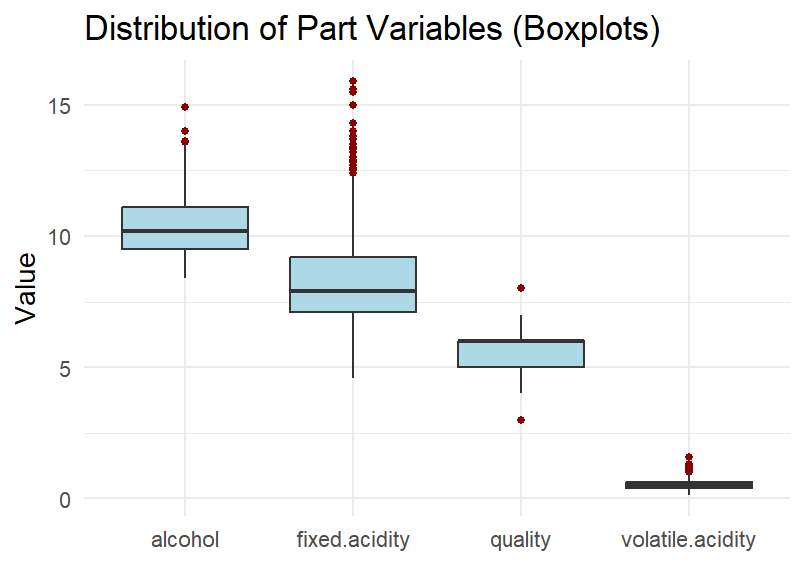
\includegraphics[width=0.5\linewidth]{../plots/bp1} 

}

\caption{Boxplot of part Variables}\label{fig:fig-box}
\end{figure}

\begin{figure}[H]

{\centering 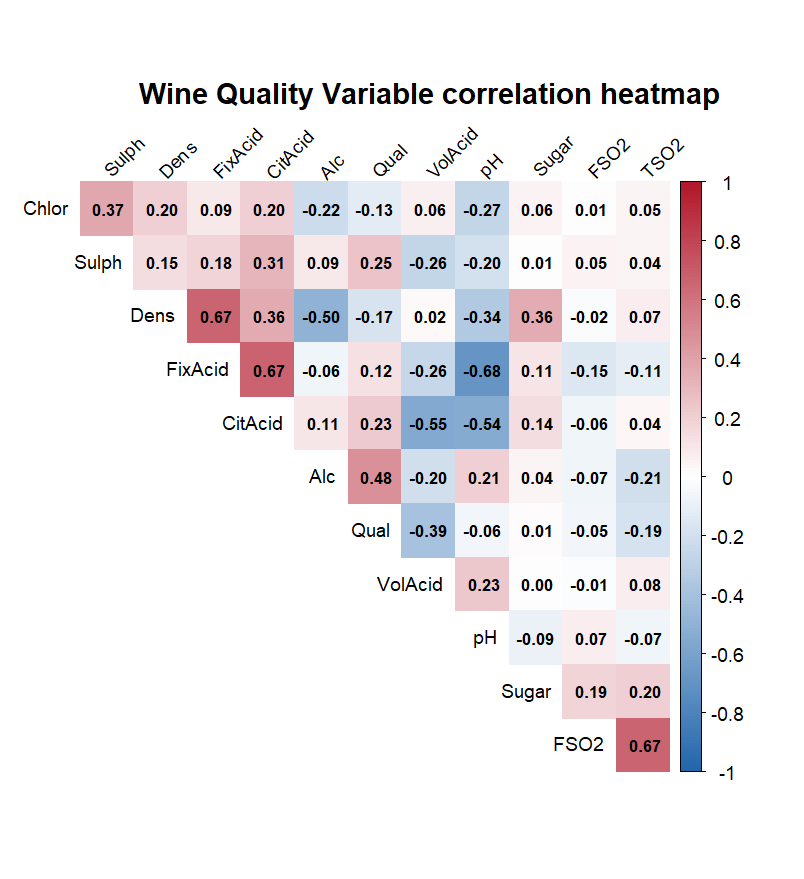
\includegraphics[width=0.5\linewidth]{../plots/r1} 

}

\caption{Heatmap of correlations between variables}\label{fig:heat}
\end{figure}

Figure 2 shows the Pearson correlation coefficient matrix of all eleven variables and the dependent variable wine quality. From the figure, we can see that alcohol and taste show a strong positive correlation (r ≈ +0.48), which indicates that wines with higher alcohol content tend to get higher quality scores. On the other hand, volatile acidity is significantly negatively correlated with health (r ≈ -0.39), indicating that the higher the volatile acidity, the lower the quality score of the wine. We also found that there may be some multicollinearity between the predictors - free SO2 and total SO2 (r = +0.67) and fixed acidity and density (r = +0.67). In short, based on this figure, we have a deeper understanding of the data, and the conclusions we get will help guide the subsequent OLS and Lasso regression methods.

\begin{figure}[H]

{\centering 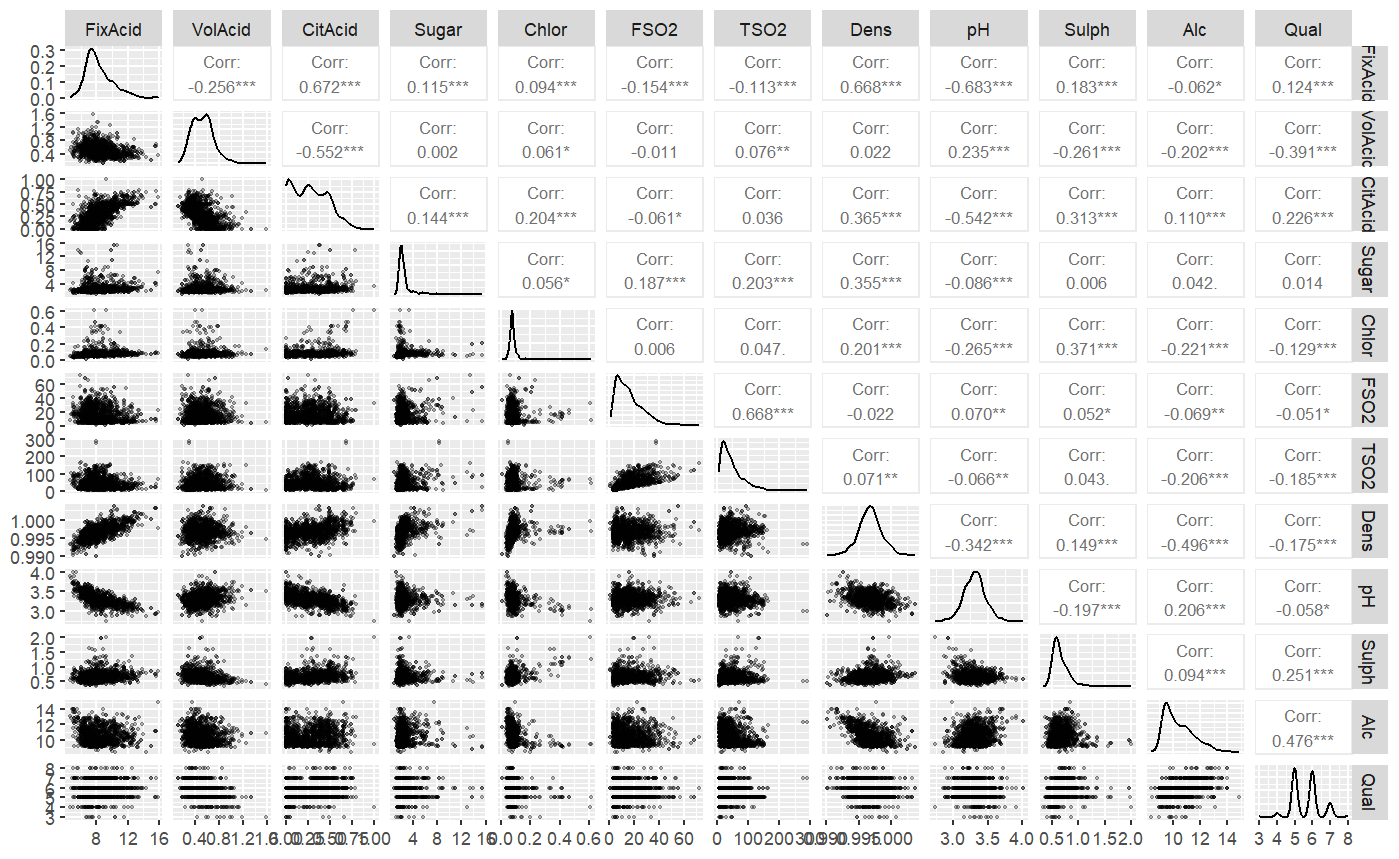
\includegraphics[width=0.5\linewidth]{../plots/p1} 

}

\caption{Pairwise Scatterplot Matrix for all variables}\label{fig:Pairwise}
\end{figure}

Figure 3 uses GGally::ggpairs to output the Pairwise Scatterplot Matrix, where the lower left corner of the diagonal outputs the scatter plots between the variables. From the scatter plots of the variables, we can see that the points of Fixed Acidity and Density are dense and distributed in an upward diagonal, reflecting the conclusion drawn from the heat map that the two variables may be highly collinear. The output in the middle of the diagonal is the kernel density estimates of each variable's marginal distribution, and the output in the upper right corner of the diagonal is the same Pearson correlation coefficient as the heat map. The smooth density curves of each variable reveal the distribution characteristics: for example, Sugar shows an obvious right-skewed long-tail distribution, while Density is highly concentrated in the range of 0.997--0.998. This matrix not only further confirms the known strong associations such as Sulphates and Quality, but also once again shows the multicollinearity problem and the abnormal marginal distribution of some variables, providing a key basis for variable screening and diagnosis of subsequent regression models.

\newpage

\section{4 Methodology \& Results}\label{methodology-results}

\subsection{4.1 Ordinary Least Squares Model (OLS)}\label{ordinary-least-squares-model-ols}

I first used the OLS model to linearly model the dependent variable wine quality for all 11 variables. The regression equation is as follows:
\begin{equation}
\label{eq:ols}
\mathrm{Qual}_i
= \beta_0
+ \beta_1\,\mathrm{FixAcid}_i
+ \beta_2\,\mathrm{VolAcid}_i
+ \cdots
+ \beta_{11}\,\mathrm{Alc}_i
+ \varepsilon_i,
\quad
\varepsilon_i \sim N(0,\sigma^2).
\end{equation}

Hypothesis tests are performed on the parameters to test the significance of the parameters. The results can be obtained from the P-value column in Table 3. For each regression coefficient \(\beta_j\), test:

Null Hypothesis(\(H_0\)) : \(\beta_j\) = 0 vs Alternative Hypothesis(\(H_a\)) : at least one \(\beta_j\) \(≠\) 0

Calculate the \(t\) statistic \(t_j = \hat\beta_j / \mathrm{SE}(\hat\beta_j)\) and report the two-tailed \(p\) value. The results show:

\begin{table}[H]

\begin{center}
\begin{threeparttable}

\caption{\label{tab:ols-model}OLS regression coefficient estimation and significance test}

\begin{tabular}{lllll}
\toprule
 & \multicolumn{1}{c}{Estimate} & \multicolumn{1}{c}{Std. Error} & \multicolumn{1}{c}{t value} & \multicolumn{1}{c}{Pr(>|t|)}\\
\midrule
(Intercept) & 21.97 & 21.19 & 1.04 & 0.30\\
FixAcid & 0.02 & 0.03 & 0.96 & 0.34\\
VolAcid & -1.08 & 0.12 & -8.95 & 0.00\\
CitAcid & -0.18 & 0.15 & -1.24 & 0.21\\
Sugar & 0.02 & 0.02 & 1.09 & 0.28\\
Chlor & -1.87 & 0.42 & -4.47 & 0.00\\
FSO2 & 0.00 & 0.00 & 2.01 & 0.04\\
TSO2 & 0.00 & 0.00 & -4.48 & 0.00\\
Dens & -17.88 & 21.63 & -0.83 & 0.41\\
pH & -0.41 & 0.19 & -2.16 & 0.03\\
Sulph & 0.92 & 0.11 & 8.01 & 0.00\\
Alc & 0.28 & 0.03 & 10.43 & 0.00\\
\bottomrule
\end{tabular}

\end{threeparttable}
\end{center}

\end{table}

Among them, we can find that the parameters of volatile acidity, chloride, total \(SO_2\), free \(SO_2\), pH, sulphates and alcohol are significant in the model, while other variables are not significant at the 5\% level. We can preliminarily conclude that these variables shown as significant above have a certain effect on the quality score of red wine. The fitting results of the OLS model show that the coefficient of determination \(R^2 = 0.3606\) indicates that the model can explain about 36.1\% of the total variance of the quality score. However, after adjustment, \(R^2\) = 0.3561, and the F statistic of the model = 81.35 (df = 11, 1587), \(p<2.2\times10^{-16}\), rejecting the null hypothesis, indicating that the model is significant.

After that, the OLS model residuals were further tested using the diagnosis() function in the library (ds4ling). The following is the output of the OLS residual model diagnostic graph:

\begin{figure}[H]

{\centering 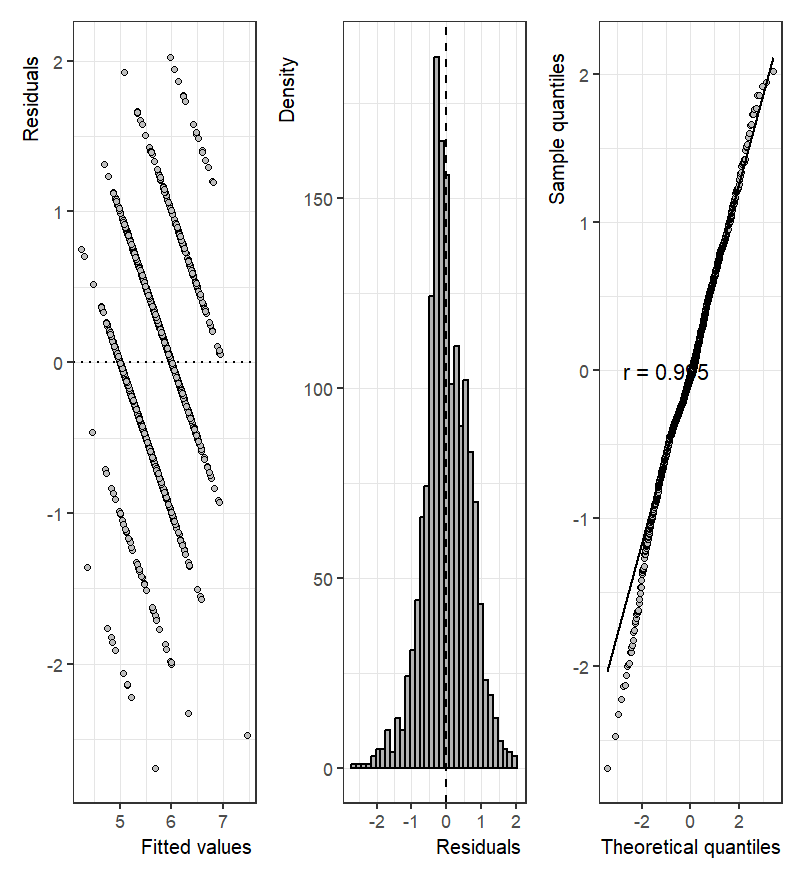
\includegraphics[width=0.5\linewidth]{../plots/OLS_res} 

}

\caption{Residual diagnosis for OLS model}\label{fig:fig-ols-res}
\end{figure}

The residuals vs.~fitted values plot on the left of the test plot shows randomly distributed scatter with no particularly obvious pattern, so the assumption of linearity can be considered supported. However, since the variance seems to increase with the fitted values, there may be slight heteroskedasticity. The Q-Q plot on the right shows that the residuals are roughly distributed along the diagonal (r = 0.95), indicating approximate normality. However, the slight deviation in the tails shows that there may be slight non-normality. The residual density plot in the middle is centered at zero and has a single peak, which is similar to the residual density plot of a good model fit, and is bell-shaped, but a slight skewness is observed.

\subsection{4.2 Lasso Regression}\label{lasso-regression}

To mitigate multicollinearity and enforce sparsity in our predictor set, we fit a Lasso model using the \textbf{glmnet} package. In matrix notation, letting \(x_i\) denote the \(p\)-dimensional predictor vector for observation \(i\) and \(y_i\) its quality score, the Lasso estimate solves

\begin{equation}
\label{eq:lasso}
\min_{\beta_0,\beta}
  \frac{1}{N}\sum_{i=1}^N \bigl(y_i - \beta_0 - x_i^\top \beta\bigr)^2
  \;+\;
  \lambda \sum_{j=1}^p \lvert \beta_j\rvert,
\quad
\lambda \ge 0.
\end{equation}

Prior to fitting, all predictors were standardized and an intercept term retained.

\subsubsection{Lambda Selection via 10-Fold Cross-Validation}\label{lambda-selection-via-10-fold-cross-validation}

Using the glmnet() function, with the penalty parameter \(α\) set to 1, we can get a complete Lasso model. We continue to set the response to the quality of the wine, and the dependent variable is the remaining 11 variables. We hope to use the Lasso model to delete as many unimportant variables as possible, making the model parameters simpler - that is, to get a sparse model. This way, we can more clearly understand which physical and chemical properties (variables) have a more significant impact on the quality of the wine.We then output a plot of \(Log(λ)\) and Mean Square Error to help determine the optimal \(λ\) value.

\begin{figure}[H]

{\centering 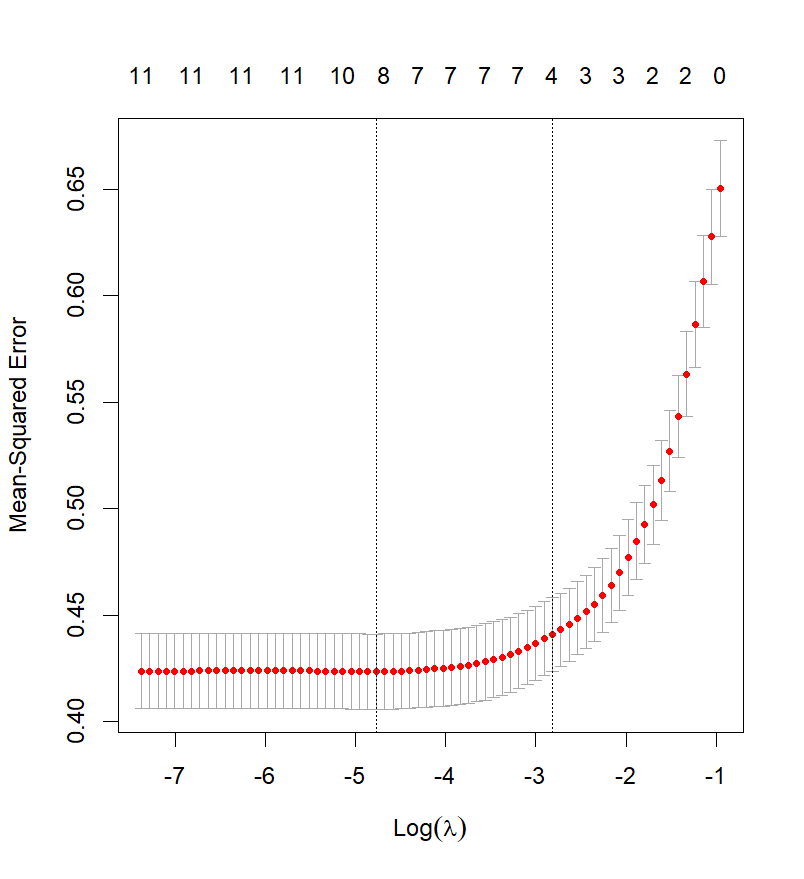
\includegraphics[width=0.5\linewidth]{../plots/cv_lasso} 

}

\caption{Plot of CV\_Lasso}\label{fig:fig-cv-lasso}
\end{figure}

The figure shows that as \(Log(λ)\) increases from -7 to -1, the MSE of the model also increases. To prevent overfitting, we believe that \(Log(λ)\) = -3 is the best value, because reducing \(Log(λ)\) further will penalize the model too much and delete some necessary parameters. The number at the top (11 to 0) indicates the number of factors with non-zero coefficients. As \(λ\) increases, fewer predictors are selected, thereby reducing the complexity of the model. At this optimal \(λ\), Lasso retains the following 8 non-zero coefficients.

Compute the cross-validation MSE for a sequence of \(λ\) values. The value (denoted as \(λ_{min}\)) that minimizes the CV error is found to be.
\(\hatλ_{min}\) = 0.00848

\begin{table}[!h]
\centering
\caption{\label{tab:lasso-coef-table}Non-zero Lasso coefficients at \(\hat{\lambda}_{\min}\)}
\centering
\begin{tabular}[t]{l|l}
\hline
term & estimate\\
\hline
(Intercept) & 4.1628\\
\hline
VolAcid & -1.0243\\
\hline
Sugar & 0.0013\\
\hline
Chlor & -1.7093\\
\hline
FSO2 & 0.0024\\
\hline
TSO2 & -0.0027\\
\hline
pH & -0.3825\\
\hline
Sulph & 0.8196\\
\hline
Alc & 0.2852\\
\hline
\end{tabular}
\end{table}
\newpage

Three predictors:fixed acidity, citric acid, and density are driven exactly to zero, indicating minimal marginal contribution once penalization is applied. The retained coefficients largely mirror OLS signs and magnitudes, reaffirming volatile acidity and chlorides as the negative drivers of quality and sulphates and alcohol content as positive drivers.

Afterwards, I used 10-fold cross validation to compare the prediction performance of OLS and Lasso models.

\begin{figure}[H]

{\centering 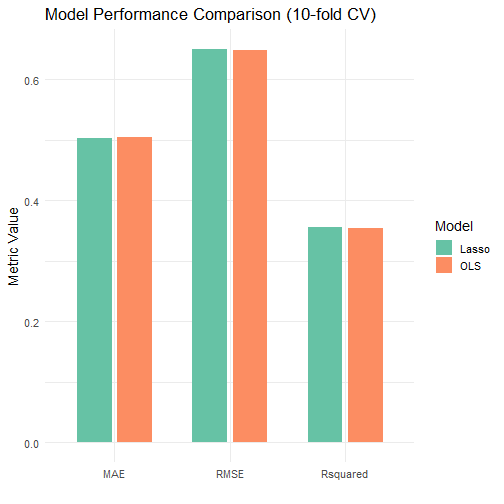
\includegraphics[width=0.5\linewidth]{../plots/cp1} 

}

\caption{OLS and Lasso Model Performance Comparison}\label{fig:figcp}
\end{figure}

From the comparison of the 10-fold cross validation of the two models, it can be seen that LASSO and OLS perform similarly in predicting wine quality, with little difference in MAE, RMSE, and R².

\subsection{5.3 Bayesian Cumulative Logit Regression}\label{bayesian-cumulative-logit-regression}

To account for the ordinal nature of our quality scores (3--8), we replace the Gaussian assumption with a Bayesian cumulative logit model, using the brms package. This framework estimates cutpoints (intercepts) that partition the latent propensity into the seven observed quality levels, and slopes for each predictor, with full posterior uncertainty.
\textbf{Model specification}
\[
\Pr\bigl(\text{Qual}_i \le k \mid x_i\bigr)
=\mathrm{logit}^{-1}\bigl(\gamma_k - x_i^\top\beta\bigr),
\quad k = 1,\dots,7,
\]
where \(\gamma_1<\gamma_2<\cdots<\gamma_7\) are the cutpoints and \(\beta\) the vector of slopes. Priors:

\[
\beta_j \sim \mathrm{Normal}(0,1),\quad 
\gamma_k \sim \mathrm{Normal}(0,5).
\]

The model was fit with four NUTS chains, 2,000 iterations each (1,000 warmup), yielding 4,000 post--warmup draws.

\subsubsection{\texorpdfstring{\textbf{Posterior summary \& convergence}}{Posterior summary \& convergence}}\label{posterior-summary-convergence}

Table 5 reports posterior medians, standard deviations, and 95\% credible intervals for each slope. Convergence diagnostics are excellent (\(\widehat R = 1.00\), Bulk ESS \& Tail ESS \textgreater1,500), though 83 divergent transitions suggest increasing \texttt{adapt\_delta} in future work.

\begin{table}[H]

\begin{center}
\begin{threeparttable}

\caption{\label{tab:bayes-summary}Posterior medians, standard deviations, and 95\textbackslash{}\% CIs for the Bayesian cumulative logit model}

\begin{tabular}{llllllll}
\toprule
 & \multicolumn{1}{c}{Estimate} & \multicolumn{1}{c}{Est.Error} & \multicolumn{1}{c}{l-95\% CI} & \multicolumn{1}{c}{u-95\% CI} & \multicolumn{1}{c}{Rhat} & \multicolumn{1}{c}{Bulk\_ESS} & \multicolumn{1}{c}{Tail\_ESS}\\
\midrule
Intercept[1] & -4.01 & 2.77 & -9.71 & 1.21 & 1.00 & 1,624.69 & 1,479.60\\
Intercept[2] & -2.29 & 2.40 & -7.02 & 2.25 & 1.00 & 2,843.95 & 2,430.04\\
Intercept[3] & 0.97 & 2.05 & -3.04 & 5.01 & 1.00 & 3,344.90 & 2,709.81\\
Intercept[4] & 2.86 & 2.02 & -1.12 & 6.77 & 1.00 & 3,322.67 & 2,507.98\\
Intercept[5] & 6.52 & 2.02 & 2.57 & 10.44 & 1.00 & 3,294.96 & 2,520.03\\
Intercept[6] & 9.32 & 2.04 & 5.34 & 13.23 & 1.00 & 3,263.36 & 2,585.26\\
Intercept[7] & 12.31 & 2.05 & 8.31 & 16.23 & 1.00 & 3,268.48 & 2,550.20\\
FixAcid & 0.08 & 0.05 & -0.01 & 0.17 & 1.00 & 2,419.76 & 2,664.06\\
VolAcid & -3.17 & 0.36 & -3.88 & -2.46 & 1.00 & 2,724.61 & 1,781.00\\
CitAcid & -0.61 & 0.40 & -1.39 & 0.16 & 1.00 & 2,408.26 & 2,762.07\\
Sugar & 0.04 & 0.04 & -0.04 & 0.12 & 1.00 & 4,439.33 & 2,766.81\\
Chlor & -1.92 & 0.77 & -3.40 & -0.40 & 1.00 & 3,424.30 & 2,619.14\\
FSO2 & 0.02 & 0.01 & 0.00 & 0.03 & 1.00 & 3,819.52 & 2,975.51\\
TSO2 & -0.01 & 0.00 & -0.02 & -0.01 & 1.00 & 3,851.32 & 3,572.76\\
Dens & -0.02 & 1.03 & -2.07 & 1.94 & 1.00 & 4,693.23 & 2,546.20\\
pH & -0.80 & 0.42 & -1.63 & 0.02 & 1.00 & 2,904.98 & 2,664.17\\
Sulph & 2.24 & 0.32 & 1.62 & 2.88 & 1.00 & 3,841.10 & 2,925.55\\
Alc & 0.92 & 0.06 & 0.81 & 1.03 & 1.00 & 3,259.26 & 2,778.33\\
\bottomrule
\end{tabular}

\end{threeparttable}
\end{center}

\end{table}

Then do the Posterior predictive check for the Bayesian cumulative logit regression model. And use pp\_check() to output the diagnosis figure:

\begin{figure}[H]

{\centering 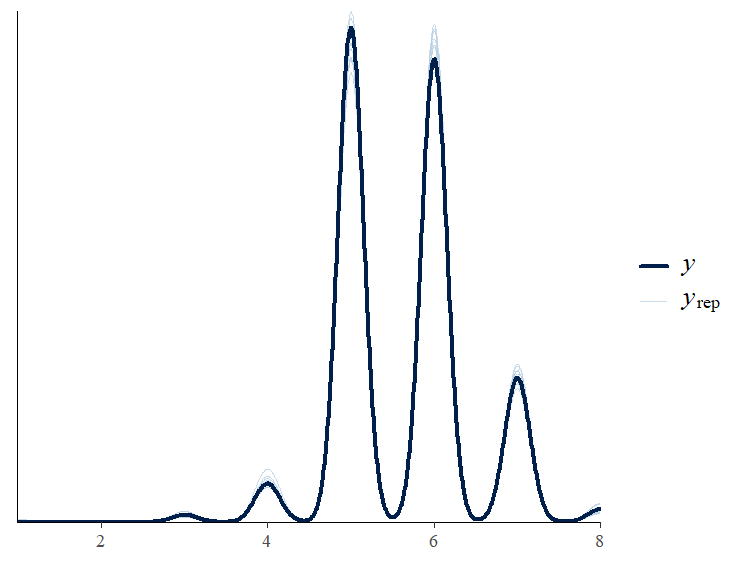
\includegraphics[width=0.6\linewidth]{../plots/kde} 

}

\caption{Posterior predictive check: observed vs. replicated quality distributions}\label{fig:ppck}
\end{figure}

Figure 7 overlays the kernel density of the observed quality distribution (\(y\), dark blue) against 10 replicated datasets (\(y_{rep}\), light blue). The replicated densities closely track the empirical peaks at scores 5, 6 and 7, demonstrating that the model captures the overall shape and modal structure of the data, with only extreme slight under‐coverage of the low (3--4) tail and large(7-8) tail.

Judging from the above analysis and diagnosis results, the ordered regression model has good convergence and the diagnosis results are relatively ideal. Volatile acid, chloride, and total SO₂ are negative influencing factors, free SO₂, sulfate, and alcohol content are positive influencing factors, and other physical and chemical characteristic indicators do not show significant effects. The Bayesian Cumulative Logit Regression model shows that the low-impact indicators that were not excluded by the previous OLS model and Lasso model only left the last 6 indicators. These indicators are considered to have a significant impact on the quality score of red wine in the three models, indicating that the Bayesian model further helps reduce unimportant indicators from a more numerically based aspect.

\subsection{5.4 Model results verification}\label{model-results-verification}

Based on the above three models, the six variables that mainly affect the quality score of red wine are given, namely volatile acid, chloride, total SO₂, free SO₂, sulfate, and alcohol content. In order to verify the discriminative ability of these six variables in evaluating the binary classification model at different thresholds, we use Logistic regression to binarize the quality of red wine. We define samples with a red wine quality score greater than or equal to 6 as ``high quality'' (HighQual=1), and the rest as ``non-high quality'' (HighQual=0). Then, a linear Logistics model is fitted and the odds ratio of each variable is calculated to further detect the positive/negative effect of each variable on the red wine quality score, as well as the intensity of the effect.

\begin{table}[H]

\begin{center}
\begin{threeparttable}

\caption{\label{tab:or-table}Odds Ratios for Logistic Regression Predictors}

\begin{tabular}{ll}
\toprule
Term & \multicolumn{1}{c}{OR}\\
\midrule
(Intercept) & 0.00\\
Alc & 2.36\\
Sulph & 14.97\\
TSO2 & 0.98\\
Chlor & 0.01\\
VolAcid & 0.06\\
FSO2 & 1.02\\
\bottomrule
\end{tabular}

\end{threeparttable}
\end{center}

\end{table}

Output table (odds table of each variable)
The model results show that alcohol and sulfate have a strong positive effect on the probability of ``high quality''. The regression coefficients of the two are significantly positive, and the corresponding odds ratios are approximately 2.36 and 14.97, respectively, indicating that under the same other conditions, the odds of high quality increase by about 136\% for every 1 percentage point increase in alcohol; the odds of high quality increase by nearly 15 times for every unit increase in sulfate. Although the marginal effect of free sulfur dioxide is small, its coefficient is also positive and significant, indicating that an appropriate amount of free SO₂ can also help improve quality evaluation. On the contrary, total sulfur dioxide, chloride and volatile acidity all show a significant inhibitory effect on the probability of high quality. The odds ratios of the three are approximately 0.98, 0.01 and 0.06, respectively, which means that their increase will correspondingly significantly reduce the probability of wine being rated as high quality, among which chloride and volatile acidity have particularly obvious negative effects.

\begin{figure}[H]

{\centering 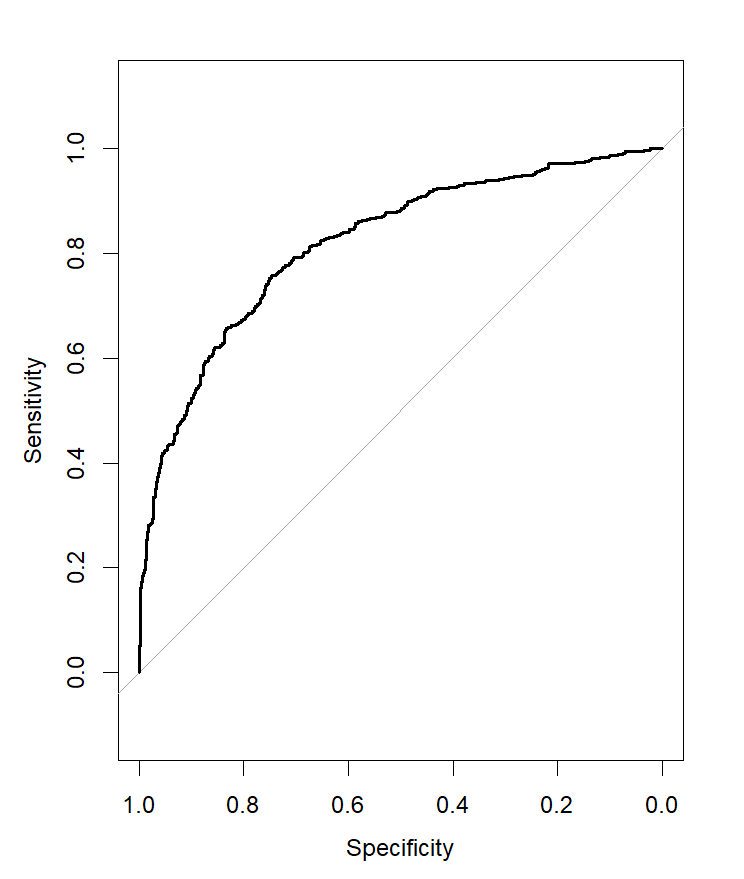
\includegraphics[width=0.6\linewidth]{../plots/ROC} 

}

\caption{ROC curve for logistic regression}\label{fig:ROC}
\end{figure}

Figure 8 shows the ROC curve output by the detection model. The curve shows a classic ``S-shaped'' trajectory from the lower left corner to the upper left corner and then to the upper right corner. It can achieve a high true positive rate (True Positive Rate \textgreater{} 0.7) in a low false positive rate range (False Positive Rate \textless{} 0.2), which shows that the model's ability to identify high-quality wines is already very good at a small error cost. The area under the curve (AUC) is 0.8188, which is greater than 0.8 and belongs to the evaluation standard of the ``good'' classification level, indicating that under all possible decision thresholds, the logistic regression model has a high stability in distinguishing the binary red wine quality scores. It should be noted that although the AUC value reflects the overall performance, it does not directly guide the selection of the optimal threshold, so in practical applications, it may be necessary to further use a more complete threshold selection method.

\section{6 Conclusion \& Future Directions}\label{conclusion-future-directions}

\subsection{6.1 Conclusion \& Discussion}\label{conclusion-discussion}

The comparison results of the three models studied above consistently show that volatile acidity, chloride, total SO₂, free SO₂, sulfate, and alcohol are the main influencing factors of red wine quality scores. In the OLS, Lasso, and Bayesian Cumulative Logit Regression models, higher alcohol is associated with an increased probability of obtaining a high-quality score, while increased volatile acidity seriously reduces the quality of red wine. Sulfate and chloride are closely followed in importance (positive values for sulfate and negative values for chloride), and total/free sulfur dioxide shows a small but credible non-zero effect in the Bayesian estimation. Other predictors (fixed acidity, citric acid, density, sugar) always produce credible intervals or confidence intervals that overlap with zero, indicating that their marginal contributions are negligible once the key drivers are considered.

The three methods differed in their handling of multicollinearity and variable selection. OLS retains all 11 slopes, but inflates standard errors when predictors are correlated (e.g., fixed acid and density, free sulfur dioxide, and total sulfur dioxide). Lasso's L1 penalty automatically shrinks small coefficients to zero, dropping fixed acid, citric acid, and density to produce a more interpretable, parsimonious model with nearly identical prediction errors (CV RMSE ≈ 0.65). In contrast, the Bayesian Cumulative Logit Regression model retains all slopes but quantifies uncertainty with 95\% credible intervals, allowing us to see which effects are credibly nonzero in an ordinal framework. This full a posteriori approach also allows for direct probabilistic descriptions of how a unit change in each predictor changes the probability of obtaining a higher quality grade.

From a production perspective, these findings have practical implications:

\begin{enumerate}
\def\labelenumi{\arabic{enumi}.}
\item
  Fermentation control: Perceived quality can be improved by selecting yeast strains or adjusting sugars to target slightly higher alcohol by volume (ABV).
\item
  Acidity management: Minimizing volatile acidity during fermentation and aging (e.g., by adding sulfur dioxide early or controlling temperature) can prevent off-flavors from disproportionately damaging sensory scores.
\item
  Finishing additives: Fine-tuning sulfate and chloride concentrations can further improve balance and mouthfeel.
  Producers can therefore focus their resources on a few factors that most reliably improve wine quality and contribute to consumers' drinking experience.
\end{enumerate}

\subsection{6.2 Limited of this study}\label{limited-of-this-study}

Limitations of this study include reliance on a single red wine dataset (UCI ``winequality-red.csv''), a cross-sectional design lacking time or regional stratification, and only discussing linear (or cumulative linear) relationships. This study did not explore potential interactions (e.g., alcohol × pH), nonlinear dose-response curves, or external sensory covariates that might further refine quality predictions.

\subsection{6.3 Future Directions}\label{future-directions}

Looking ahead, this study can be further deepened and expanded from the following aspects:
On the one hand, interaction terms and nonlinear basis expansion can be introduced into the existing model to capture the complex coupling effects and nonlinear responses between chemical properties, thereby improving the prediction accuracy;
On the other hand, a horizontal comparative analysis can be conducted on red wine samples from different production areas or years to test the versatility and robustness of the model under differences in regions, climates and cultivation conditions;
In addition, with the help of a hierarchical Bayesian framework, grouping information such as producers and production areas can be incorporated into the model hierarchy, and parameter estimation can be improved through information aggregation and ``learning by leveraging'', and the uncertainty at each level can be quantified;
At the same time, the chemical measurement data and the subjective scores obtained from the sensory evaluation panel can be organically combined to construct a chemical-sensory mapping model to further reveal the intrinsic connection between chemical indicators and human tasting experience;
Finally, other potential influencing factors (such as brewing technology, microbial community characteristics, etc.) can be introduced and modeled together with existing chemical variables, so as to comprehensively deepen the understanding of the driving mechanism of red wine quality and provide more accurate decision-making support for theoretical research and industrial practice.

\newpage

\section{References}\label{references}

\begin{itemize}
\tightlist
\item
  Montgomery, D. C., Peck, E. A., \& Vining, G. G. (2012). Introduction to linear regression analysis. Hoboken, NJ: Wiley.
\item
  Tibshirani, R. (1996). Regression shrinkage and selection via the lasso. Journal of the Royal Statistical Society: Series B (Methodological), 58(1), 267--288. Wiley.
\item
  Gelman, A., Carlin, J. B., Stern, H. S., Dunson, D. B., Vehtari, A., \& Rubin, D. B. (2013). Bayesian data analysis (3rd ed.). Boca Raton, FL: Chapman \& Hall/CRC.
\item
  Polson, N. G., Scott, J. G., \& Windle, J. (2013). Bayesian inference for logistic models using Polya--Gamma latent variables. Journal of the American Statistical Association, 108(504), 1339--1349. Taylor \& Francis.
\end{itemize}

\newpage
\appendix

\begin{Shaded}
\begin{Highlighting}[]
\CommentTok{\# Loading necessary library}
\FunctionTok{library}\NormalTok{(tidyverse)}
\FunctionTok{library}\NormalTok{(here)}
\FunctionTok{library}\NormalTok{(dplyr)}
\FunctionTok{library}\NormalTok{(tidyr)}
\FunctionTok{library}\NormalTok{(ds4ling)}
\FunctionTok{library}\NormalTok{(lme4)}
\FunctionTok{library}\NormalTok{(lmerTest)}
\FunctionTok{library}\NormalTok{(GGally)}
\FunctionTok{library}\NormalTok{(corrplot)}
\FunctionTok{library}\NormalTok{(ggcorrplot)}
\FunctionTok{library}\NormalTok{(rstanarm)}
\FunctionTok{library}\NormalTok{(brms)}
\FunctionTok{library}\NormalTok{(glmnet)}
\FunctionTok{library}\NormalTok{(caret)}
\FunctionTok{library}\NormalTok{(tibble)}

\CommentTok{\# Read the raw data}
\NormalTok{data\_wine\_raw }\OtherTok{\textless{}{-}} \FunctionTok{read.csv}\NormalTok{(}
  \FunctionTok{here}\NormalTok{(}\StringTok{"data\_raw"}\NormalTok{, }\StringTok{"winequality{-}red.csv"}\NormalTok{),}
  \AttributeTok{header =} \ConstantTok{TRUE}\NormalTok{,}
  \AttributeTok{sep =} \StringTok{";"}\NormalTok{,}
  \AttributeTok{stringsAsFactors =} \ConstantTok{FALSE}
\NormalTok{)}

\CommentTok{\# Test if there has any NA in data\_wine\_raw}
\FunctionTok{anyNA}\NormalTok{(data\_wine\_raw)}
\FunctionTok{colSums}\NormalTok{(}\FunctionTok{is.na}\NormalTok{(data\_wine\_raw))}

\CommentTok{\# View data structure}
\FunctionTok{glimpse}\NormalTok{(data\_wine\_raw)}

\FunctionTok{summary}\NormalTok{(data\_wine\_raw)}

\NormalTok{data\_wine\_tidy }\OtherTok{\textless{}{-}}\NormalTok{ data\_wine\_raw }\SpecialCharTok{\%\textgreater{}\%}
  \FunctionTok{rename}\NormalTok{(}
    \AttributeTok{FixAcid =}\NormalTok{ fixed.acidity,}
    \AttributeTok{VolAcid =}\NormalTok{ volatile.acidity,}
    \AttributeTok{CitAcid =}\NormalTok{ citric.acid,}
    \AttributeTok{Sugar   =}\NormalTok{ residual.sugar,}
    \AttributeTok{Chlor   =}\NormalTok{ chlorides,}
    \AttributeTok{FSO2    =}\NormalTok{ free.sulfur.dioxide,}
    \AttributeTok{TSO2    =}\NormalTok{ total.sulfur.dioxide,}
    \AttributeTok{Dens    =}\NormalTok{ density,}
    \AttributeTok{pH      =}\NormalTok{ pH,}
    \AttributeTok{Sulph   =}\NormalTok{ sulphates,}
    \AttributeTok{Alc     =}\NormalTok{ alcohol,}
    \AttributeTok{Qual    =}\NormalTok{ quality}
\NormalTok{  )}\SpecialCharTok{|\textgreater{}}
  \FunctionTok{write\_csv}\NormalTok{(}\StringTok{"./data\_tidy/data\_wine\_tidy.csv"}\NormalTok{)}


\CommentTok{\# dplyr summary}
\NormalTok{data\_wine\_tidy }\SpecialCharTok{|\textgreater{}}
  \FunctionTok{summarise}\NormalTok{(}\FunctionTok{across}\NormalTok{(}
    \AttributeTok{.cols =} \FunctionTok{everything}\NormalTok{(),}
    \AttributeTok{.fns =} \FunctionTok{list}\NormalTok{(}
      \AttributeTok{mean   =} \SpecialCharTok{\textasciitilde{}} \FunctionTok{mean}\NormalTok{(.x, }\AttributeTok{na.rm =} \ConstantTok{TRUE}\NormalTok{),}
      \AttributeTok{median =} \SpecialCharTok{\textasciitilde{}} \FunctionTok{median}\NormalTok{(.x, }\AttributeTok{na.rm =} \ConstantTok{TRUE}\NormalTok{),}
      \AttributeTok{Q1     =} \SpecialCharTok{\textasciitilde{}} \FunctionTok{quantile}\NormalTok{(.x, }\FloatTok{0.25}\NormalTok{, }\AttributeTok{na.rm =} \ConstantTok{TRUE}\NormalTok{),}
      \AttributeTok{Q3     =} \SpecialCharTok{\textasciitilde{}} \FunctionTok{quantile}\NormalTok{(.x, }\FloatTok{0.75}\NormalTok{, }\AttributeTok{na.rm =} \ConstantTok{TRUE}\NormalTok{)}
\NormalTok{    ),}
    \AttributeTok{.names =} \StringTok{"\{.col\}\_\{.fn\}"}
\NormalTok{  )) }\SpecialCharTok{|\textgreater{}}
  \FunctionTok{pivot\_longer}\NormalTok{(}\FunctionTok{everything}\NormalTok{(),}
               \AttributeTok{names\_to  =} \FunctionTok{c}\NormalTok{(}\StringTok{"variable"}\NormalTok{, }\StringTok{"stat"}\NormalTok{),}
               \AttributeTok{names\_sep =} \StringTok{"\_"}\NormalTok{,}
               \AttributeTok{values\_to =} \StringTok{"value"}\NormalTok{) }\SpecialCharTok{|\textgreater{}}
  \FunctionTok{arrange}\NormalTok{(variable, stat)}


\NormalTok{five\_num\_summary }\OtherTok{\textless{}{-}}\NormalTok{ data\_wine\_tidy }\SpecialCharTok{|\textgreater{}}
  \FunctionTok{summarise}\NormalTok{(}\FunctionTok{across}\NormalTok{(}
    \AttributeTok{.cols =} \FunctionTok{everything}\NormalTok{(),}
    \AttributeTok{.fns =} \FunctionTok{list}\NormalTok{(}
      \AttributeTok{Min  =} \SpecialCharTok{\textasciitilde{}} \FunctionTok{min}\NormalTok{(.x, }\AttributeTok{na.rm =} \ConstantTok{TRUE}\NormalTok{),}
      \AttributeTok{Q1   =} \SpecialCharTok{\textasciitilde{}} \FunctionTok{quantile}\NormalTok{(.x, }\FloatTok{0.25}\NormalTok{, }\AttributeTok{na.rm =} \ConstantTok{TRUE}\NormalTok{),}
      \AttributeTok{Median =} \SpecialCharTok{\textasciitilde{}} \FunctionTok{median}\NormalTok{(.x, }\AttributeTok{na.rm =} \ConstantTok{TRUE}\NormalTok{),}
      \AttributeTok{Q3   =} \SpecialCharTok{\textasciitilde{}} \FunctionTok{quantile}\NormalTok{(.x, }\FloatTok{0.75}\NormalTok{, }\AttributeTok{na.rm =} \ConstantTok{TRUE}\NormalTok{),}
      \AttributeTok{Max  =} \SpecialCharTok{\textasciitilde{}} \FunctionTok{max}\NormalTok{(.x, }\AttributeTok{na.rm =} \ConstantTok{TRUE}\NormalTok{)}
\NormalTok{    ),}
    \AttributeTok{.names =} \StringTok{"\{.col\}\_\{.fn\}"}
\NormalTok{  )) }\SpecialCharTok{|\textgreater{}}
  \FunctionTok{pivot\_longer}\NormalTok{(}\FunctionTok{everything}\NormalTok{(),}
               \AttributeTok{names\_to =} \FunctionTok{c}\NormalTok{(}\StringTok{"variable"}\NormalTok{, }\StringTok{"stat"}\NormalTok{),}
               \AttributeTok{names\_sep =} \StringTok{"\_"}\NormalTok{,}
               \AttributeTok{values\_to =} \StringTok{"value"}\NormalTok{) }\SpecialCharTok{\%\textgreater{}\%}
  \FunctionTok{pivot\_wider}\NormalTok{(}\AttributeTok{names\_from =}\NormalTok{ stat, }\AttributeTok{values\_from =}\NormalTok{ value)}

\CommentTok{\# Display the Five{-}Number Summary}
\FunctionTok{print}\NormalTok{(five\_num\_summary)}

\CommentTok{\# Create Boxplots for all variables}
\NormalTok{data\_long }\OtherTok{\textless{}{-}}\NormalTok{ data\_wine\_tidy }\SpecialCharTok{\%\textgreater{}\%}
  \FunctionTok{pivot\_longer}\NormalTok{(}
    \AttributeTok{cols =} \FunctionTok{everything}\NormalTok{(),}
    \AttributeTok{names\_to =} \StringTok{"Variable"}\NormalTok{,}
    \AttributeTok{values\_to =} \StringTok{"Value"}
\NormalTok{  )}

\FunctionTok{ggplot}\NormalTok{(data\_long, }\FunctionTok{aes}\NormalTok{(}\AttributeTok{x =}\NormalTok{ Variable, }\AttributeTok{y =}\NormalTok{ Value, }\AttributeTok{fill =}\NormalTok{ Variable)) }\SpecialCharTok{+}
  \FunctionTok{geom\_boxplot}\NormalTok{(}\AttributeTok{outlier.color =} \StringTok{"darkred"}\NormalTok{, }\AttributeTok{outlier.size =} \FloatTok{1.5}\NormalTok{) }\SpecialCharTok{+}
  \FunctionTok{labs}\NormalTok{(}
    \AttributeTok{title =} \StringTok{"Boxplots of All Variables"}\NormalTok{,}
    \AttributeTok{x =} \StringTok{"Variables"}\NormalTok{,}
    \AttributeTok{y =} \StringTok{"Value"}
\NormalTok{  ) }\SpecialCharTok{+}
  \FunctionTok{theme\_minimal}\NormalTok{(}\AttributeTok{base\_size =} \DecValTok{12}\NormalTok{) }\SpecialCharTok{+}
  \FunctionTok{theme}\NormalTok{(}\AttributeTok{axis.text.x =} \FunctionTok{element\_text}\NormalTok{(}\AttributeTok{angle =} \DecValTok{45}\NormalTok{, }\AttributeTok{hjust =} \DecValTok{1}\NormalTok{)) }\SpecialCharTok{+}
  \FunctionTok{scale\_fill\_brewer}\NormalTok{(}\AttributeTok{palette =} \StringTok{"Pastel1"}\NormalTok{) }\SpecialCharTok{+}
  \FunctionTok{theme}\NormalTok{(}\AttributeTok{legend.position =} \StringTok{"none"}\NormalTok{)}


\CommentTok{\# Select the core variables and pivot to long format}
\NormalTok{data\_core }\OtherTok{\textless{}{-}}\NormalTok{ data\_wine\_raw }\SpecialCharTok{\%\textgreater{}\%}
  \FunctionTok{select}\NormalTok{(fixed.acidity, volatile.acidity, alcohol, quality) }\SpecialCharTok{\%\textgreater{}\%}
  \FunctionTok{pivot\_longer}\NormalTok{(}
    \AttributeTok{cols =} \FunctionTok{everything}\NormalTok{(),}
    \AttributeTok{names\_to  =} \StringTok{"Variable"}\NormalTok{,}
    \AttributeTok{values\_to =} \StringTok{"Value"}
\NormalTok{  )}

\CommentTok{\# Plot boxplots for core variables}
\FunctionTok{ggplot}\NormalTok{(data\_core, }\FunctionTok{aes}\NormalTok{(}\AttributeTok{x =}\NormalTok{ Variable, }\AttributeTok{y =}\NormalTok{ Value)) }\SpecialCharTok{+}
  \FunctionTok{geom\_boxplot}\NormalTok{(}\AttributeTok{fill =} \StringTok{"lightblue"}\NormalTok{, }\AttributeTok{outlier.color =} \StringTok{"darkred"}\NormalTok{) }\SpecialCharTok{+}
  \FunctionTok{labs}\NormalTok{(}
    \AttributeTok{title =} \StringTok{"Distribution of Part Variables (Boxplots)"}\NormalTok{,}
    \AttributeTok{x     =} \ConstantTok{NULL}\NormalTok{,}
    \AttributeTok{y     =} \StringTok{"Value"}
\NormalTok{  ) }\SpecialCharTok{+}
  \FunctionTok{theme\_minimal}\NormalTok{(}\AttributeTok{base\_size =} \DecValTok{14}\NormalTok{)}

\CommentTok{\# Variable correlation heatmap}
\CommentTok{\# Calculate correlation matrix}
\NormalTok{corr\_mat }\OtherTok{\textless{}{-}} \FunctionTok{cor}\NormalTok{(data\_wine\_tidy, }\AttributeTok{use =} \StringTok{"pairwise.complete.obs"}\NormalTok{)}

\CommentTok{\# Generate a gradient color from blue to white to red}
\NormalTok{my\_col }\OtherTok{\textless{}{-}} \FunctionTok{colorRampPalette}\NormalTok{(}\FunctionTok{c}\NormalTok{(}\StringTok{"\#2166AC"}\NormalTok{, }\StringTok{"white"}\NormalTok{, }\StringTok{"\#B2182B"}\NormalTok{))(}\DecValTok{200}\NormalTok{)}

\FunctionTok{corrplot}\NormalTok{(}
\NormalTok{  corr\_mat,}
  \AttributeTok{method      =} \StringTok{"color"}\NormalTok{,}
  \AttributeTok{col         =}\NormalTok{ my\_col,}
  \AttributeTok{type        =} \StringTok{"upper"}\NormalTok{,}
  \AttributeTok{order       =} \StringTok{"hclust"}\NormalTok{,}
  \AttributeTok{tl.col      =} \StringTok{"black"}\NormalTok{, }
  \AttributeTok{tl.srt      =} \DecValTok{45}\NormalTok{,}
  \AttributeTok{tl.cex      =} \FloatTok{0.8}\NormalTok{,}
  \AttributeTok{addCoef.col =} \StringTok{"black"}\NormalTok{,}
  \AttributeTok{number.cex  =} \FloatTok{0.7}\NormalTok{,}
  \AttributeTok{diag        =} \ConstantTok{FALSE}\NormalTok{,}
  \AttributeTok{mar         =} \FunctionTok{c}\NormalTok{(}\DecValTok{0}\NormalTok{,}\DecValTok{0}\NormalTok{,}\DecValTok{1}\NormalTok{,}\DecValTok{0}\NormalTok{)}
\NormalTok{)}
\FunctionTok{title}\NormalTok{(}\StringTok{"Wine Quality Variable correlation heatmap"}\NormalTok{, }\AttributeTok{line =} \FloatTok{0.5}\NormalTok{, }\AttributeTok{cex.main =} \FloatTok{1.2}\NormalTok{)}


\CommentTok{\#Pairwise scatterplot matrix}

\NormalTok{GGally}\SpecialCharTok{::}\FunctionTok{ggpairs}\NormalTok{(}
\NormalTok{  data\_wine\_tidy,}
  \AttributeTok{lower =} \FunctionTok{list}\NormalTok{(}\AttributeTok{continuous =} \FunctionTok{wrap}\NormalTok{(}\StringTok{"points"}\NormalTok{, }\AttributeTok{alpha =} \FloatTok{0.3}\NormalTok{, }\AttributeTok{size =} \FloatTok{0.5}\NormalTok{)),}
  \AttributeTok{upper =} \FunctionTok{list}\NormalTok{(}\AttributeTok{continuous =} \FunctionTok{wrap}\NormalTok{(}\StringTok{"cor"}\NormalTok{, }\AttributeTok{size =} \DecValTok{3}\NormalTok{)),}
  \AttributeTok{diag  =} \FunctionTok{list}\NormalTok{(}\AttributeTok{continuous =} \FunctionTok{wrap}\NormalTok{(}\StringTok{"densityDiag"}\NormalTok{))}
\NormalTok{)}

\CommentTok{\# 6. Ordinary Least Squares Regression (OLS)}
\NormalTok{model\_ols }\OtherTok{\textless{}{-}} \FunctionTok{lm}\NormalTok{(Qual }\SpecialCharTok{\textasciitilde{}}\NormalTok{ ., }\AttributeTok{data =}\NormalTok{ data\_wine\_tidy)}
\FunctionTok{summary}\NormalTok{(model\_ols)}


\FunctionTok{diagnosis}\NormalTok{(model\_ols)}

\CommentTok{\# Fit the Lasso regression}
\NormalTok{x }\OtherTok{\textless{}{-}} \FunctionTok{model.matrix}\NormalTok{(Qual }\SpecialCharTok{\textasciitilde{}}\NormalTok{ ., }\AttributeTok{data =}\NormalTok{ data\_wine\_tidy)[, }\SpecialCharTok{{-}}\DecValTok{1}\NormalTok{]}
\NormalTok{y }\OtherTok{\textless{}{-}}\NormalTok{ data\_wine\_tidy}\SpecialCharTok{$}\NormalTok{Qual}

\CommentTok{\# 10{-}fold cross{-}validation to find optimal λ}
\FunctionTok{set.seed}\NormalTok{(}\DecValTok{2025}\NormalTok{)}
\NormalTok{cv\_lasso }\OtherTok{\textless{}{-}} \FunctionTok{cv.glmnet}\NormalTok{(x, y, }\AttributeTok{alpha =} \DecValTok{1}\NormalTok{, }\AttributeTok{family =} \StringTok{"gaussian"}\NormalTok{, }\AttributeTok{standardize =} \ConstantTok{TRUE}\NormalTok{, }\AttributeTok{nfolds =} \DecValTok{10}\NormalTok{)}
\FunctionTok{plot}\NormalTok{(cv\_lasso)}
\NormalTok{best\_lambda }\OtherTok{\textless{}{-}}\NormalTok{ cv\_lasso}\SpecialCharTok{$}\NormalTok{lambda.min}
\NormalTok{best\_lambda}

\CommentTok{\# Extract coefficients}
\NormalTok{lasso\_coef }\OtherTok{\textless{}{-}} \FunctionTok{coef}\NormalTok{(cv\_lasso, }\AttributeTok{s =} \StringTok{"lambda.min"}\NormalTok{)}
\FunctionTok{print}\NormalTok{(lasso\_coef)}

\CommentTok{\# Model performance comparison}
\FunctionTok{set.seed}\NormalTok{(}\DecValTok{2025}\NormalTok{)}
\NormalTok{train\_ctrl }\OtherTok{\textless{}{-}} \FunctionTok{trainControl}\NormalTok{(}\AttributeTok{method =} \StringTok{"cv"}\NormalTok{, }\AttributeTok{number =} \DecValTok{10}\NormalTok{)}

\CommentTok{\# OLS CV}
\NormalTok{ols\_cv }\OtherTok{\textless{}{-}} \FunctionTok{train}\NormalTok{(}
\NormalTok{  Qual }\SpecialCharTok{\textasciitilde{}}\NormalTok{ .,}
  \AttributeTok{data      =}\NormalTok{ data\_wine\_tidy,}
  \AttributeTok{method    =} \StringTok{"lm"}\NormalTok{,}
  \AttributeTok{trControl =}\NormalTok{ train\_ctrl}
\NormalTok{)}

\CommentTok{\# Lasso CV}
\NormalTok{lasso\_cv }\OtherTok{\textless{}{-}} \FunctionTok{train}\NormalTok{(}
\NormalTok{  Qual }\SpecialCharTok{\textasciitilde{}}\NormalTok{ .,}
  \AttributeTok{data      =}\NormalTok{ data\_wine\_tidy,}
  \AttributeTok{method    =} \StringTok{"glmnet"}\NormalTok{,}
  \AttributeTok{trControl =}\NormalTok{ train\_ctrl,}
  \AttributeTok{tuneGrid  =} \FunctionTok{expand.grid}\NormalTok{(}\AttributeTok{alpha =} \DecValTok{1}\NormalTok{, }\AttributeTok{lambda =}\NormalTok{ cv\_lasso}\SpecialCharTok{$}\NormalTok{lambda)}
\NormalTok{)}

\CommentTok{\# Output model performance}
\NormalTok{ols\_cv}
\NormalTok{lasso\_cv}



\CommentTok{\#Fit the Bayes model }
\NormalTok{priors }\OtherTok{\textless{}{-}} \FunctionTok{c}\NormalTok{(}
  \FunctionTok{set\_prior}\NormalTok{(}\StringTok{"normal(0, 1)"}\NormalTok{, }\AttributeTok{class =} \StringTok{"b"}\NormalTok{),}
  \FunctionTok{set\_prior}\NormalTok{(}\StringTok{"normal(0, 5)"}\NormalTok{, }\AttributeTok{class =} \StringTok{"Intercept"}\NormalTok{)}
\NormalTok{)}

\NormalTok{model\_bayes }\OtherTok{\textless{}{-}} \FunctionTok{brm}\NormalTok{(}
\NormalTok{  Qual }\SpecialCharTok{\textasciitilde{}}\NormalTok{ .,}
  \AttributeTok{data            =}\NormalTok{ data\_wine\_tidy,}
  \AttributeTok{family          =} \FunctionTok{cumulative}\NormalTok{(}\AttributeTok{link =} \StringTok{"logit"}\NormalTok{),}
  \AttributeTok{prior           =}\NormalTok{ priors,}
  \AttributeTok{chains          =} \DecValTok{4}\NormalTok{,}
  \AttributeTok{cores           =}\NormalTok{ parallel}\SpecialCharTok{::}\FunctionTok{detectCores}\NormalTok{(),}
  \AttributeTok{iter            =} \DecValTok{2000}\NormalTok{,}
  \AttributeTok{seed            =} \DecValTok{2025}
\NormalTok{)}

\FunctionTok{print}\NormalTok{(model\_bayes, }\AttributeTok{digits =} \DecValTok{2}\NormalTok{)}

\CommentTok{\# 9.2 Posterior intervals}
\FunctionTok{posterior\_interval}\NormalTok{(model\_bayes, }\AttributeTok{prob =} \FloatTok{0.95}\NormalTok{)}

\CommentTok{\# 9.3 Posterior predictive check}
\FunctionTok{pp\_check}\NormalTok{(model\_bayes)}




\CommentTok{\# Binarize: Qual \textgreater{}= 6 as 1, otherwise 0}
\NormalTok{data\_wine\_tidy }\OtherTok{\textless{}{-}}\NormalTok{ data\_wine\_tidy }\SpecialCharTok{|\textgreater{}}
  \FunctionTok{mutate}\NormalTok{(}\AttributeTok{HighQual =} \FunctionTok{if\_else}\NormalTok{(Qual }\SpecialCharTok{\textgreater{}=} \DecValTok{6}\NormalTok{, }\DecValTok{1}\NormalTok{, }\DecValTok{0}\NormalTok{))}

\CommentTok{\# Logistic regression}
\NormalTok{model\_logit }\OtherTok{\textless{}{-}} \FunctionTok{glm}\NormalTok{(}
  \AttributeTok{formula =}\NormalTok{ HighQual }\SpecialCharTok{\textasciitilde{}}\NormalTok{ Alc }\SpecialCharTok{+}\NormalTok{ Sulph }\SpecialCharTok{+}\NormalTok{ TSO2 }\SpecialCharTok{+}\NormalTok{ Chlor }\SpecialCharTok{+}\NormalTok{ VolAcid }\SpecialCharTok{+}\NormalTok{ FSO2,}
  \AttributeTok{data    =}\NormalTok{ data\_wine\_tidy,}
  \AttributeTok{family  =} \FunctionTok{binomial}\NormalTok{(}\AttributeTok{link =} \StringTok{"logit"}\NormalTok{)}
\NormalTok{)}

\FunctionTok{summary}\NormalTok{(model\_logit)}

\CommentTok{\# Calculate odds ratios}
\FunctionTok{exp}\NormalTok{(}\FunctionTok{coef}\NormalTok{(model\_logit))}

\CommentTok{\# Predict probabilities \& ROC}
\FunctionTok{library}\NormalTok{(pROC)}
\NormalTok{pred\_prob }\OtherTok{\textless{}{-}} \FunctionTok{predict}\NormalTok{(model\_logit, }\AttributeTok{type =} \StringTok{"response"}\NormalTok{)}
\NormalTok{roc\_obj   }\OtherTok{\textless{}{-}} \FunctionTok{roc}\NormalTok{(data\_wine\_tidy}\SpecialCharTok{$}\NormalTok{HighQual, pred\_prob)}
\FunctionTok{plot}\NormalTok{(roc\_obj); }\FunctionTok{auc}\NormalTok{(roc\_obj)}
\end{Highlighting}
\end{Shaded}


\end{document}
